% Methodology diagram: FBR + CDAN+E + Mean Teacher.
% Standalone: compile with `tectonic pipeline_fbr_cdane_mt.tex` (or pdflatex).
% In the paper: 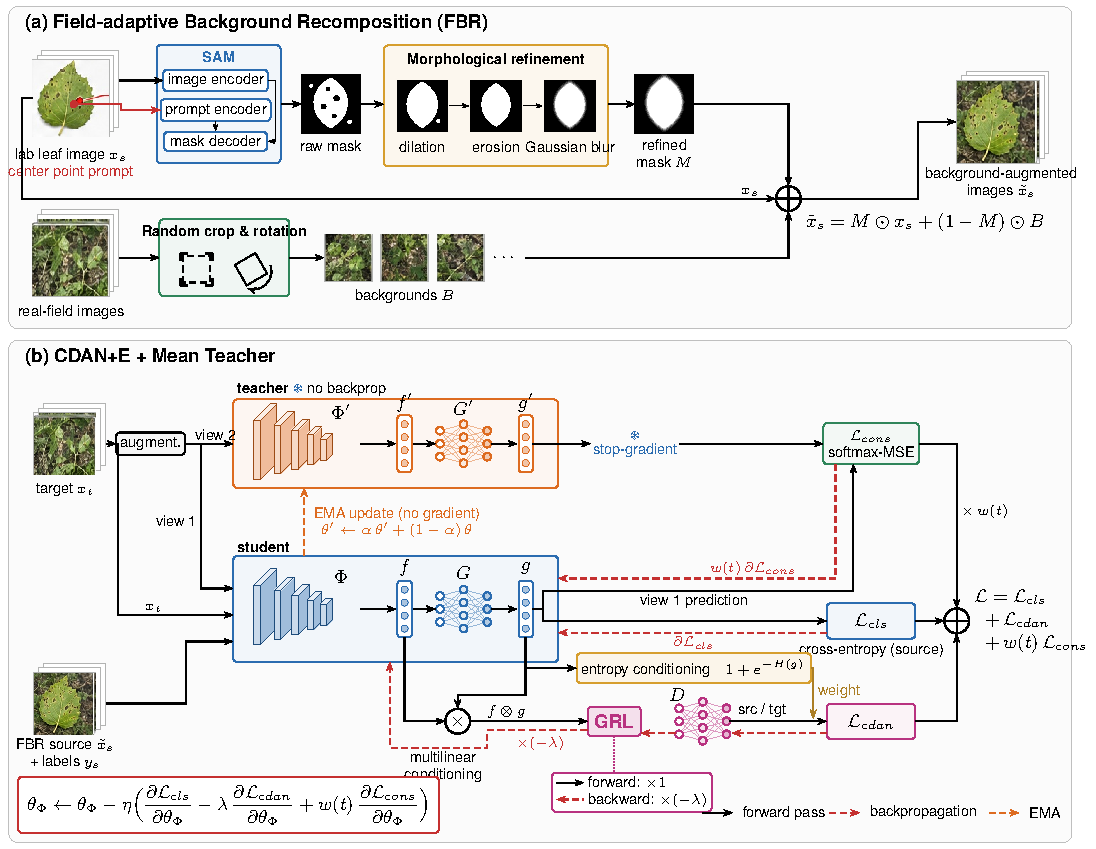
\includegraphics[width=\textwidth]{pipeline_fbr_cdane_mt.pdf}
% Photos are read from img/; replace them with real dataset samples.
\documentclass[tikz,border=3pt]{standalone}
\usepackage[T1]{fontenc}
\usepackage{helvet}
\renewcommand{\familydefault}{\sfdefault}
\usepackage{amsmath,amssymb,bm}
\usepackage{pifont}
\usetikzlibrary{arrows.meta,calc,positioning}

% ---------------------------------------------------------------- palette
\definecolor{srcc}{HTML}{2B6CB0}   % source / student
\definecolor{tgtc}{HTML}{2F855A}   % target / field
\definecolor{tchc}{HTML}{DD6B20}   % teacher / EMA
\definecolor{grlc}{HTML}{B83280}   % GRL / adversarial
\definecolor{gradc}{HTML}{C53030}  % backpropagation
\definecolor{fbrc}{HTML}{D69E2E}   % morphology / entropy

\tikzset{
  >={Stealth[length=4pt,width=3pt]},
  fwd/.style={->,line width=0.6pt},
  bwd/.style={->,gradc,densely dashed,line width=0.65pt},
  ema/.style={->,tchc,densely dashed,line width=0.7pt},
  blk/.style={draw,rounded corners=2pt,line width=0.5pt,font=\scriptsize,align=center,inner sep=2pt},
  lbl/.style={font=\scriptsize,align=center,inner sep=1pt},
  ptitle/.style={anchor=west,font=\bfseries\small},
  loss/.style={blk,minimum width=1.5cm,minimum height=0.6cm,font=\small},
}

% \photo{x}{y}{size}{file}: square image thumbnail
\newcommand{\photo}[4]{%
  \node[inner sep=0,draw=gray!60,line width=0.4pt] at (#1,#2)
    {\includegraphics[width=#3cm,height=#3cm]{img/#4}};}
% \stackphoto{x}{y}{size}{file}: thumbnail with two cards behind (= a set)
\newcommand{\stackphoto}[4]{%
  \foreach \o in {0.16,0.08}{
    \filldraw[fill=white,draw=gray!60,line width=0.4pt]
      ($(#1,#2)+(\o-#3/2,\o-#3/2)$) rectangle ++(#3,#3);}
  \photo{#1}{#2}{#3}{#4}}

% leaf silhouette in unit coordinates
\newcommand{\leafshape}{(0,-0.40) .. controls (0.40,-0.18) and (0.36,0.26) .. (0,0.44)
  .. controls (-0.36,0.26) and (-0.40,-0.18) .. (0,-0.40) -- cycle}
% \maskthumb{x}{y}{size}{kind}: 0 raw, 1 dilated, 2 eroded, 3 soft (blurred)
\newcommand{\maskthumb}[4]{%
  \begin{scope}[shift={(#1,#2)}]
    \fill[black] (-#3/2,-#3/2) rectangle (#3/2,#3/2);
    \begin{scope}[scale=#3]
      \ifcase#4
        \fill[white] \leafshape;
        \fill[black] (0.10,0.10) circle (0.045) (-0.12,-0.04) circle (0.04)
                     (0.06,-0.20) circle (0.03) (-0.05,0.26) circle (0.03);
        \fill[white] (0.32,-0.30) circle (0.03) (-0.33,0.31) circle (0.022);
      \or
        \fill[white,scale=1.07] \leafshape;
        \fill[white] (0.32,-0.30) circle (0.03);
      \or
        \fill[white] \leafshape;
      \or
        \foreach \s/\op in {1.17/0.12,1.12/0.22,1.07/0.38,1.03/0.6}
          {\fill[white,opacity=\op,scale=\s] \leafshape;}
        \fill[white] \leafshape;
      \fi
    \end{scope}
  \end{scope}}

% \cnn{x}{y}{color}: CNN drawn as shrinking feature-map slabs (left edge at x)
\newcommand{\cnn}[3]{%
  \begin{scope}[shift={(#1,#2)}]
    \foreach \x/\h in {0/1.0,0.34/0.82,0.64/0.66,0.90/0.50,1.12/0.36}{
      \pgfmathsetmacro{\d}{0.28*\h}
      \filldraw[fill=#3!45,draw=#3!70!black,line width=0.3pt]
        (\x+0.11,-\h/2) -- (\x+0.11+\d,-\h/2+\d) -- (\x+0.11+\d,\h/2+\d) -- (\x+0.11,\h/2) -- cycle;
      \filldraw[fill=#3!12,draw=#3!70!black,line width=0.3pt]
        (\x,\h/2) -- (\x+\d,\h/2+\d) -- (\x+0.11+\d,\h/2+\d) -- (\x+0.11,\h/2) -- cycle;
      \filldraw[fill=#3!25,draw=#3!70!black,line width=0.3pt]
        (\x,-\h/2) rectangle (\x+0.11,\h/2);}
  \end{scope}}

% \fcnet{x}{y}{color}: small fully connected network (3-4-3 neurons)
\newcommand{\fcnet}[3]{%
  \begin{scope}[shift={(#1,#2)}]
    \foreach \a in {-0.22,0,0.22}{\foreach \b in {-0.33,-0.11,0.11,0.33}{
      \draw[#3!50,line width=0.25pt] (-0.4,\a) -- (0,\b) -- (0.4,\a);}}
    \foreach \a in {-0.22,0,0.22}{
      \filldraw[fill=white,draw=#3,line width=0.5pt] (-0.4,\a) circle (0.065);
      \filldraw[fill=#3!35,draw=#3,line width=0.5pt] (0.4,\a) circle (0.065);}
    \foreach \b in {-0.33,-0.11,0.11,0.33}
      {\filldraw[fill=#3!15,draw=#3,line width=0.5pt] (0,\b) circle (0.065);}
  \end{scope}}

% \fvec{x}{y}{color}: feature / prediction vector
\newcommand{\fvec}[3]{%
  \begin{scope}[shift={(#1,#2)}]
    \filldraw[fill=white,draw=#3,rounded corners=1.5pt,line width=0.5pt]
      (-0.12,-0.48) rectangle (0.12,0.48);
    \foreach \b in {-0.33,-0.11,0.11,0.33}
      {\filldraw[fill=#3!40,draw=#3,line width=0.4pt] (0,\b) circle (0.06);}
  \end{scope}}

% \network{y}{color}{prime}: Phi -> f -> G -> g, x positions shared by student/teacher
\newcommand{\network}[3]{%
  \cnn{4.15}{#1-0.1}{#2}
  \fvec{6.7}{#1}{#2}
  \fcnet{7.7}{#1}{#2}
  \fvec{8.75}{#1}{#2}
  \draw[fwd,line width=0.5pt] (5.95,#1) -- (6.55,#1);
  \draw[fwd,line width=0.5pt] (6.85,#1) -- (7.22,#1);
  \draw[fwd,line width=0.5pt] (8.18,#1) -- (8.6,#1);
  \node[lbl,font=\small] at (5.62,#1+0.55) {$\Phi#3$};
  \node[lbl,font=\small] at (6.7,#1+0.7) {$f#3$};
  \node[lbl,font=\small] at (7.7,#1+0.62) {$G#3$};
  \node[lbl,font=\small] at (8.75,#1+0.7) {$g#3$};}

% \oplusnode{name}{x}{y}
\newcommand{\oplusnode}[3]{%
  \node[circle,draw,fill=white,line width=0.7pt,minimum size=0.42cm,inner sep=0] (#1) at (#2,#3) {};
  \draw[line width=0.7pt] (#1.north) -- (#1.south) (#1.west) -- (#1.east);}

\begin{document}
\begin{tikzpicture}

% =====================================================================
% (a) FBR
% =====================================================================
\begin{scope}[yshift=0.75cm]
  \filldraw[fill=gray!3,draw=gray!50,rounded corners=4pt] (0,7.95) rectangle (18,13.4);
  \node[ptitle] at (0.15,13.12) {(a) Field-adaptive Background Recomposition (FBR)};

  % --- lab image + SAM
  \stackphoto{1.05}{11.85}{1.3}{lab_leaf.png}
  \fill[gradc] (1.1,11.75) circle (0.06);
  \node[lbl] at (1.05,10.88) {lab leaf image $x_s$};
  \node[lbl,text=gradc] at (1.05,10.6) {center point prompt};

  \node[blk,draw=srcc,fill=srcc!6,minimum width=2.1cm,minimum height=2.0cm] (sam) at (3.55,11.75) {};
  \node[lbl,font=\bfseries\scriptsize,text=srcc] at (3.55,12.55) {SAM};
  \node[blk,draw=srcc,fill=white,minimum width=1.75cm,minimum height=0.32cm] (ienc) at (3.5,12.15) {image encoder};
  \node[blk,draw=srcc,fill=white,minimum width=1.75cm,minimum height=0.32cm] (penc) at (3.5,11.65) {prompt encoder};
  \node[blk,draw=srcc,fill=white,minimum width=1.75cm,minimum height=0.32cm] (mdec) at (3.5,11.12) {mask decoder};
  \draw[fwd] (1.88,12.15) -- (ienc.west);
  \draw[->,gradc,line width=0.6pt] (1.1,11.75) -- (1.9,11.75) |- (penc.west);
  \draw[->,line width=0.4pt] (penc.south) -- (mdec.north);
  \draw[->,line width=0.4pt] (ienc.east) -- ++(0.12,0) |- (mdec.east);

  % --- raw mask -> morphological refinement -> refined mask M
  \maskthumb{5.45}{11.75}{1.0}{0}
  \node[lbl] at (5.45,11.05) {raw mask};
  \draw[fwd] (sam.east) -- (4.95,11.75);

  \node[blk,draw=fbrc,fill=fbrc!8,minimum width=3.8cm,minimum height=2.05cm] (morph) at (8.25,11.72) {};
  \node[lbl,font=\bfseries\scriptsize] at (8.25,12.5) {Morphological refinement};
  \maskthumb{7.0}{11.72}{0.85}{1}
  \maskthumb{8.25}{11.72}{0.85}{2}
  \maskthumb{9.5}{11.72}{0.85}{3}
  \node[lbl] at (7.0,11.03) {dilation};
  \node[lbl] at (8.25,11.03) {erosion};
  \node[lbl] at (9.5,11.03) {Gaussian blur};
  \draw[fwd,line width=0.45pt] (7.46,11.72) -- (7.8,11.72);
  \draw[fwd,line width=0.45pt] (8.71,11.72) -- (9.05,11.72);
  \draw[fwd] (5.95,11.75) -- (morph.west |- 0,11.75);

  \maskthumb{11.1}{11.75}{1.0}{3}
  \node[lbl] at (11.1,10.92) {refined\\mask $M$};
  \draw[fwd] (morph.east |- 0,11.75) -- (10.6,11.75);

  % --- field image -> random crop & rotation -> backgrounds B
  \stackphoto{1.05}{9.15}{1.3}{field.png}
  \node[lbl] at (1.05,8.22) {real-field images};

  \node[blk,draw=tgtc,fill=tgtc!7,minimum width=2.2cm,minimum height=1.3cm] (crop) at (3.65,9.15) {};
  \node[lbl,font=\bfseries\scriptsize] at (3.65,9.58) {Random crop \& rotation};
  \draw[densely dashed,line width=0.5pt] (2.95,8.73) rectangle (3.4,9.18);
  \foreach \sx/\sy in {1/1,1/-1,-1/1,-1/-1}
    {\draw[line width=0.9pt] ($(3.175,8.955)+(\sx*0.27,\sy*0.27)$) -- ++(-\sx*0.12,0)
       ($(3.175,8.955)+(\sx*0.27,\sy*0.27)$) -- ++(0,-\sy*0.12);}
  \draw[line width=0.5pt,rotate around={30:(4.1,8.955)}] (3.9,8.755) rectangle (4.3,9.155);
  \draw[->,line width=0.6pt] (4.43,9.02) arc (20:-110:0.3);
  \draw[fwd] (1.88,9.15) -- (crop.west);

  \photo{5.75}{9.15}{0.8}{bg1.png}
  \photo{6.7}{9.15}{0.8}{bg2.png}
  \photo{7.65}{9.15}{0.8}{bg3.png}
  \node[font=\small] at (8.4,9.15) {$\cdots$};
  \node[lbl] at (6.7,8.5) {backgrounds $B$};
  \draw[fwd] (crop.east) -- (5.33,9.15);

  % --- alpha compositing
  \oplusnode{plus}{13.2}{10.15}
  \draw[fwd] (11.6,11.75) -| (plus.north);
  \draw[fwd] (0.4,11.85) -- (0.22,11.85) |- (plus.west);
  \node[lbl,anchor=south] at (12.55,10.15) {$x_s$};
  \draw[fwd] (8.75,9.15) -| (plus.south);
  \node[anchor=north west,font=\small,inner sep=1pt] at (13.45,9.95)
    {$\tilde{x}_s = M \odot x_s + (1-M) \odot B$};

  \stackphoto{16.75}{11.45}{1.4}{fbr_out.png}
  \draw[fwd] (plus.east) -- (15.4,10.15) |- (16.03,11.45);
  \node[lbl] at (16.8,10.42) {background-augmented\\images $\tilde{x}_s$};
\end{scope}

% =====================================================================
% (b) CDAN+E + Mean Teacher
% =====================================================================
\filldraw[fill=gray!3,draw=gray!50,rounded corners=4pt] (0,0) rectangle (18,8.5);
\node[ptitle] at (0.15,8.22) {(b) CDAN+E + Mean Teacher};

% --- inputs
\stackphoto{0.95}{6.75}{1.05}{field.png}
\node[lbl] at (0.95,5.98) {target $x_t$};
\node[blk,fill=gray!8,minimum width=0.95cm,minimum height=0.38cm] (aug) at (2.4,6.75) {augment.};
\draw[fwd] (1.65,6.75) -- (aug.west);

\stackphoto{0.95}{2.35}{1.05}{fbr_out.png}
\node[lbl] at (0.95,1.5) {FBR source $\tilde{x}_s$\\+ labels $y_s$};

% --- teacher
\node[blk,draw=tchc,fill=tchc!6,minimum width=5.5cm,minimum height=1.5cm] (teacher) at (6.55,6.75) {};
\node[anchor=south west,font=\scriptsize,inner sep=1pt] at (3.82,7.52)
  {\textbf{teacher} \textcolor{srcc}{\ding{100}} no backprop};
\network{6.75}{tchc}{'}

% --- student
\node[blk,draw=srcc,fill=srcc!6,minimum width=5.5cm,minimum height=1.8cm] (student) at (6.55,3.95) {};
\node[anchor=south west,font=\scriptsize,inner sep=1pt] at (3.82,4.87) {\textbf{student}};
\network{3.95}{srcc}{}

% --- input routing
\draw[fwd] (aug.east) -- (teacher.west |- 0,6.75);
\node[lbl,anchor=south] at (3.5,6.77) {view 2};
\draw[fwd] (3.25,6.75) |- (student.west |- 0,4.3);
\node[lbl,anchor=east] at (3.22,5.45) {view 1};
\draw[fwd] (1.85,6.75) |- (student.west |- 0,3.85);
\node[lbl,anchor=south] at (2.45,3.86) {$x_t$};
\draw[fwd] (1.65,2.35) -- (3.0,2.35) |- (student.west |- 0,3.4);

% --- EMA
\draw[ema] (5.0,4.85) -- (5.0,6.0);
\node[lbl,anchor=west,text=tchc] at (5.12,5.42)
  {EMA update (no gradient)\\$\theta' \leftarrow \alpha\,\theta' + (1-\alpha)\,\theta$};

% --- losses (right column)
\node[loss,draw=tgtc,fill=tgtc!6,minimum height=0.7cm,font=\scriptsize] (lcons) at (14.6,6.75)
  {$\mathcal{L}_{cons}$\\softmax-MSE};
\node[loss,draw=srcc,fill=srcc!6] (lcls) at (14.6,3.75) {$\mathcal{L}_{cls}$};
\node[lbl,anchor=north] at (14.6,3.42) {cross-entropy (source)};
\node[loss,draw=grlc,fill=grlc!6] (lcdan) at (14.6,2.05) {$\mathcal{L}_{cdan}$};

% teacher -> stop-gradient -> L_cons
\node[lbl,text=srcc] (sg) at (10.6,6.75) {\ding{100}\\[-1pt]stop-gradient};
\draw[fwd] (8.87,6.75) -- (sg.west);
\draw[fwd] (sg.east) -- (lcons.west);

% student -> L_cls and L_cons
\draw[line width=0.6pt] (8.87,3.95) -- (9.05,3.95);
\draw[fwd] (9.05,3.95) |- (lcls.west |- 0,3.75);
\draw[fwd] (9.05,3.95) |- (14.3,4.25) -- (14.3,6.4);
\node[lbl,anchor=north] at (11.6,4.23) {view 1 prediction};

% backpropagation into the student
\draw[bwd] (14.0,6.4) -- (14.0,4.47) -- (student.east |- 0,4.47);
\node[lbl,anchor=south,text=gradc] at (12.6,4.47) {$w(t)\,\partial\mathcal{L}_{cons}$};
\draw[bwd] (lcls.west |- 0,3.55) -- (student.east |- 0,3.55);
\node[lbl,anchor=north,text=gradc] at (11.6,3.53) {$\partial\mathcal{L}_{cls}$};

% --- CDAN+E branch
\node[circle,draw,fill=white,line width=0.7pt,minimum size=0.42cm,inner sep=0,font=\small] (otimes) at (7.6,2.05) {$\times$};
\draw[fwd] (6.7,3.47) |- (otimes.west);
\draw[fwd] (8.75,3.47) -- (8.75,2.5) -| (otimes.north);
\node[lbl] at (7.35,1.28) {multilinear\\conditioning};
\node[lbl,anchor=south west] at (8.05,2.07) {$f \otimes g$};

\node[blk,draw=fbrc,fill=fbrc!10,minimum height=0.5cm] (ent) at (11.6,2.95)
  {entropy conditioning\quad$1+e^{-H(g)}$\,};
\draw[fwd] (8.75,2.95) -- (ent.west);

\node[blk,draw=grlc,fill=grlc!15,minimum width=0.9cm,minimum height=0.5cm,font=\bfseries\small,text=grlc] (grl) at (10.25,2.05) {GRL};
\draw[fwd] (otimes.east) -- (grl.west);

\fcnet{11.75}{2.05}{grlc}
\node[lbl,font=\small] at (11.32,2.5) {$D$};
\draw[fwd] (12.2,2.05) -- (lcdan.west);
\node[lbl,anchor=south] at (12.75,2.07) {src / tgt};
\draw[fwd,fbrc!80!black] (ent.east) -| (13.62,2.1);
\node[lbl,anchor=west,text=fbrc!80!black] at (13.66,2.56) {weight};

% backpropagation through D and the GRL
\draw[bwd] (lcdan.west |- 0,1.85) -- (12.25,1.85);
\draw[bwd] (11.28,1.85) -- (grl.east |- 0,1.85);
\draw[bwd] (grl.west |- 0,1.9) -- (8.1,1.9) -- (8.1,1.6) -- (6.45,1.6) -- (6.45,3.05);
\node[lbl,text=gradc,font=\scriptsize\bfseries] at (9.0,1.68) {$\times(-\lambda)$};

% GRL inset
\node[blk,draw=grlc,fill=white,align=left,font=\scriptsize] (grlin) at (10.55,0.85) {%
  \tikz[baseline=-0.6ex]\draw[->,line width=0.6pt] (0,0) -- (0.45,0); forward: $\times 1$\\
  \tikz[baseline=-0.6ex]\draw[<-,gradc,densely dashed,line width=0.6pt] (0,0) -- (0.45,0); backward: $\times(-\lambda)$};
\draw[grlc,densely dotted,line width=0.5pt] (grl.south) -- (grl.south |- grlin.north);

% --- total loss
\oplusnode{total}{16.05}{3.75}
\draw[fwd] (lcls.east) -- (total.west);
\draw[fwd] (lcons.east) -| (total.north);
\node[lbl,anchor=west] at (16.08,5.6) {$\times\,w(t)$};
\draw[fwd] (lcdan.east) -| (total.south);
\node[anchor=west,font=\small,align=left,inner sep=1pt] at (16.3,3.75)
  {$\mathcal{L} = \mathcal{L}_{cls}$\\$\;\;+\,\mathcal{L}_{cdan}$\\$\;\;+\,w(t)\,\mathcal{L}_{cons}$};

% --- parameter update of the feature extractor
\node[blk,draw=gradc,fill=white,anchor=south west,font=\small,inner sep=4pt] at (0.15,0.15)
  {$\theta_\Phi \leftarrow \theta_\Phi - \eta\Big(\dfrac{\partial\mathcal{L}_{cls}}{\partial\theta_\Phi}
    - \lambda\,\dfrac{\partial\mathcal{L}_{cdan}}{\partial\theta_\Phi}
    + w(t)\,\dfrac{\partial\mathcal{L}_{cons}}{\partial\theta_\Phi}\Big)$};

% --- legend
\begin{scope}[shift={(11.75,0.5)},font=\scriptsize]
  \draw[fwd] (0,0) -- (0.5,0);  \node[anchor=west] at (0.55,0) {forward pass};
  \draw[bwd] (2.15,0) -- (2.65,0); \node[anchor=west] at (2.7,0) {backpropagation};
  \draw[ema] (4.85,0) -- (5.35,0);  \node[anchor=west] at (5.4,0) {EMA};
\end{scope}

\end{tikzpicture}
\end{document}
